\chapter{Methods}

This chapter introduces the system architecture followed by the experimental designs for the quantitative analysis. The system architecture describes the GNU Radio flow-graph description and the software and hardware used in this project. The experiments are presented in chronological order. In the first experiment, the performance of the system is measured with respect to broader parameters like sampling rate, data payload size and the number of message sent per second. The second experiment was designed was look at the impact of these parameters on the the different subsections of the data path. Then, the experiments are more focused on the USB Bus transfer. In experiment 3, the project looks at the impact of the size of the bus transfer on the overall delay. Finally the modifications introduced in hardware and software are introduced. It is followed by the the experimentation on the impact of finer bus transfer size and the GNU radio buffer sizes on the overall round trip times and how the process utilizes the system resources.

\section{System Architecture}
The experimental system is primarily based on the WIME project implementation of 802.15.4 protocol. It is adapted to use the LimeSDR board instead of USRP as the \ac{sdr} platform. The adaptations can be grouped as

\begin{enumerate}
\item{GNU Radio blocks}
\item{802.15.4 \ac{PHY} layer}
\item{Periodic Message Source}
\end{enumerate}

\paragraph{GNU Radio Blocks}

For using the LimeSDR platform the USRP Sink and Source blocks are replaced by the grlimesdr project source and sink blocks. Another alternate used in this project is the gr-osmosdr project sink and source blocks which used soapysdr to access the Lime API. The former was chosen as it directly interacts with the LimeAPI without using the adaptation layer presented by the soapysdr project. This gives much better control of the board control parameters and also saves subsequent memcpy operations used by the soapysdr glue layer. (\textbf{Maybe present the RTT values for using the two different blocks and show that the limesdr block is better.}

)

\paragraph{802.15.4 \ac{PHY} layer}

The WIME project \ac{PHY} layer has been designed to only work with 4 MHz as the sampling rate, in this project, the \ac{PHY} layer has been modified to accommodate different sampling rates. \textbf{Describe the change}

\textbf{Describe the timing probe}
\paragraph{Periodic Message Source}

A periodic message source block was implemented in the GNU Radio, it takes in the message length and time period as parameters. Figure \ref{message_source} shows the working of the message source with respect to time. The data length controls the duty cycle of the signal by varying $\Delta T_{tx}$, which is the time is requires to transmit the message through USB.\\

The block notes down the global system time as $T_1$ when it publishes a message to its output port. When the block receives the message the time $T_1$ is written to a file for analysis with the reception time measured in the \ac{PHY} layer. As only valid messages are received by this block writing $T_1$ only on valid receive helps in measuring the time delay only for valid data points.\\

Since the time noted should be compared with those from usbmon, \textit{gettimeofday} was selected as the preferred method. The time period was set such that the transmitted message is received before sending the next message.\\

\begin{figure}[h!]
\centering
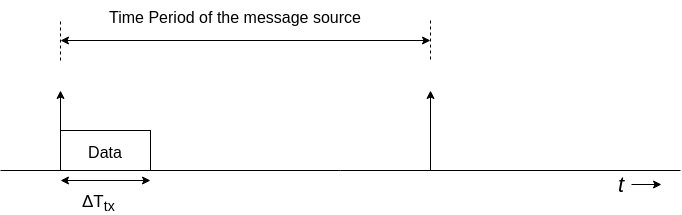
\includegraphics[width=\textwidth]{Figure/Message_Source.png}
\caption{Periodic Message Source}
\label{message_source}
\end{figure}


\subsection{System Description}

\begin{figure}[h!]
\centering
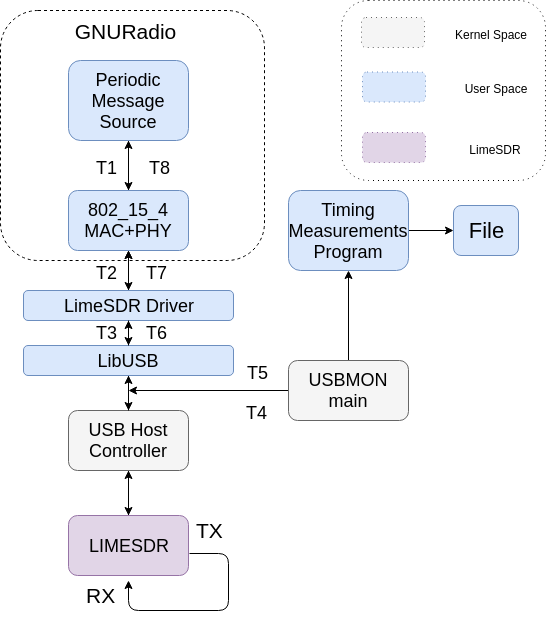
\includegraphics[width=0.8\textwidth]{Figure/Setup2.png}
\caption{System Description}
\label{setup_overview}
\end{figure}

\subsection{Software Description}
\subsection{Hardware Description}
\section{Timing Analysis}

The project uses the Wime Project implementation of 802.15.4 MAC and PHY layers in GNU Radio. For the purpose of measurement of round trip latency, a loop back experimentation setup(Figure \ref{setup_overview}) was implemented. A periodic message source generates messages and notes down the time T1. It is then processed and modulated by the 802.15.4 MAC and PHY respectively and sent through the OSMOCOM transreceiver to the LimeSDR. The RX and TX ports of the LMS7002M has been shorted and hence the original sent message loopbacks through the FPGA and comes back to the GNU Radio and is demodulated and processed by the PHY and MAC blocks respectively and is ultimately received by the periodic message source and the time is noted as T4.

The usbmon kernel utility continuously monitors bus activity between the LimeSDR USB driver and USB Host Controller. It timestamps the transfers and generates event queues to be accessed from the user space. The timing measurements program parses the event queue to find the relevant packets and notes down their usbmon timestamps as T3 and T4 for transmit and receive packets respectively.  
\subsection{Message Source} \label{message_source}

\subsection{Timing Measurements Program}
The timing measurements program uses ioctl to access the /dev/usbmonX character device. This allows the program to access the usbmon kernel utility event queue. The events are filtered to find packets with \textbf{0x01} \& \textbf{0x81} device endpoints. The data streams are parsed to find the relevant data fields from FPGA packets(Figure \ref{fpga_packet}), following that the data is converted from integer representation to complex floating point representation. The modulus of In Phase Sample's amplitude is used to determine if the data contained in the packet is useful or not. 

\begin{table}
\centering
\begin{tabular}{|c|c|}
\hline
USB Transfer Direction & Threshold Value  \\
\hline
|I| TX & 0.8\\
|I| RX & 0.2\\
\hline
\end{tabular}
\caption{Transfer Direction and Threshold Value}
\label{thres_table}
\end{table}

Analyzing the samples in the data stream, the samples threshold for actual data packets to as shown in Table \ref{thres_table}.  Once the packets have been analyzed, the sequence of events was studied to generate a state machine representation for the timing functionality.\\ 
The sequence follows the structure shown in figure \ref{sequence} if the condition mentioned about the time period in \ref{message_source} is satisfied. Since we want to measure the round trip delay, the time instant of the first TX and last RX packet as noted by T2 and T3 respectively needs to be measured. The difference between them gives the Kernel round-trip delay as measured by usbmon.    
\begin{figure}[h!]
\centering
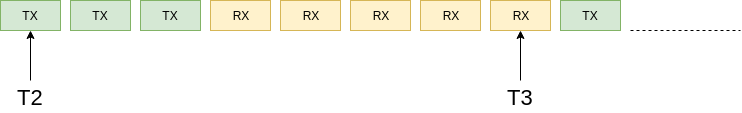
\includegraphics[width=\textwidth]{Figure/Sequence.png}
\caption{Sequence of valid data packet with time}
\label{sequence}
\end{figure}
\begin{figure}[h!]
\centering
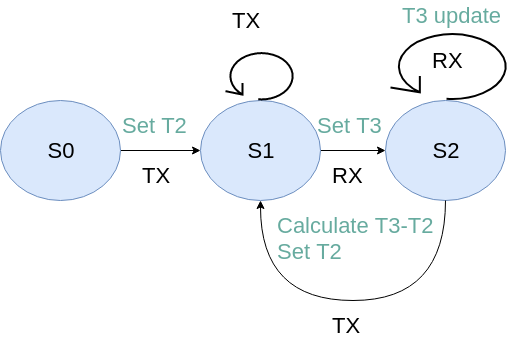
\includegraphics[scale=0.5]{Figure/State_Machine.png}
\caption{State Machine}
\label{state_machine}
\end{figure}

State Machine shown in Figure \ref{state_machine} controls the timing measurement function. It starts with state S0 and when it receives a TX event it sets T2 and moves to S1, further TX events don't update the value of T2 as we want the first TX event time. The state machine moves from S1 to S2 on a RX event, it sets the value of T3, further RX events updates the value of T3 as we want the time instant of the last RX event. On receiving TX event when at S2, it moves to S1, calculates $T3-T2$ and sets the value of T2.
\subsection{Results Correlation Method}
All the time instants are stored in Unix Time Format, a python script stores the values in separate arrays t1, t2, t3, t4 for GNU Radio Transmit Time, Kernel Transmit Time, Kernel Receive Time and GNU Radio Receive Time respectively. 

\begin{algorithm}[!h]
\caption{Time Data Correlation}
\begin{algorithmic}
\State {$T \gets $ Time Period of Message Source }
\State {$l \gets $ min(length of time arrays)}
\State $i \gets 0$
\For {$i < l $}
\If{($ t1[i]> t2[i]$ or $ t3[i]> t4[i]$)} \\
\hspace{1.35cm} delete $t1[i],t4[i]$
\ElsIf{$(t2[i]-t1[i]) > T $}
delete t2[i]
\ElsIf{$(t4[i]-t3[i]) > T $}
delete t3[i] 
\Else{ $i \gets i+1$ \\ \hspace{1.35cm} $l \gets $ min(length of time arrays) }
\EndIf
\EndFor
\end{algorithmic}
\end{algorithm}

Once the arrays have been compared to remove corrupt data, the mean and standard deviation of the respective arrays are found.
